\chapter{Background}
\section{Introduction}

\subsection{Semantic clone definition}



A code fragment in the source code that is identical, or similar, to another code fragment in the code base is considered code clone to the second and both called clone pair. This definition is based on concept of similarity. Within existing literature, the following categorization of clone definition have been widely acceptable:  



\begin{description}
	
	
	
	\item [Type I:] Identical code fragments except for variations in
	
	whitespace (may also have variations in layout) and comments. 
	
	
	
	\item[Type II:] Structurally/syntactically identical fragments except for
	
	variations in identifiers, literals, types, layout and comments.
	
	
	
	\item [Type III:] Copied fragments with further modifications.
	
	Statements can be changed, added or removed in addition to
	
	variations in identifiers, literals, types, layout and comments.
	
	
	
	%\item Functional Similarity: If the functionalities of the two code fragments are identical or similar i.e., they have similar pre and post conditions, we call them semantic clones \cite{KomondoorRaghavan03ProcedureEx, KrinkeJens01PDG, MishneGilad04Retrieval, DaveyNeil95Development} and referred as {\em Type IV} clones.
	
	
	
	\item [Type IV:] Two or more code fragments that
	
	perform the same computation but are implemented through different
	
	syntactic variants. 
	
	
	
\end{description}



Type I, Type II, and Type III clones are based on textual similarity. A code's fragments are considers clones if they are textually similar, even if they are functionally different. Textual clones are more common in software code base because they are usually the result of copy/paste practice. Conversely, functional similar code fragments are considered clones even they are textually (syntactically) different. Semantic clones are difficult to detect since they could be implemented by different syntactics and any single change in a code fragment could change the meaning (functionality) of the fragment.

%The term semantic clone, or functionally similar clones

Type IV clones (some times referred  to as functional clones or dependence clones)  are the results of semantic similarity between two or more code fragments. In this type of clones, the cloned fragment is not sharing the syntax of structure from the original. Two code fragments could be developed by two different programmers to do the same kind of task, making the code fragments similar in their functionality. The best example for semantic clones are sorting algorithms (merge sort, quick sort, and bubble sort). All of them do the same functionality and are implemented in a different ways, syntactic, and structure. To simplify, the following two functions do the same logic (swapping two variables). However, implemented in two different  syntactic.


%\lstset{style=sharpc}
\begin{lstlisting}
public static int[] swap(int[] a, int i, int j)
{
int x = a[i];
a[i] = a[j];
a[j] = x;
return a;
}

public static int[] swapNoTemp(int[] a, int i, int j)
{
a[i] = a[i]+a[j];
a[j] = a[i]-a[j];
a[i] = a[i]-a[j];
return a;
}

\end{lstlisting}

Some practitioners consider syntactic clones that have similar functionality to be semantic clones while others define semantic clones as functionally similar and syntactically different. \cite{Roy2007} defines semantic clones as a functionally similar clones and implemented using a different syntactics; while \cite{Davey1995,Elva2013, Elva2012} consider functionally similar code fragments as a semantic clones regardless of its syntactic. 



They key challenge is to detect  (semantic) clones that are not detectable by the most mature syntactic detectors such as: NICAD \cite{Roy2008}, CCFinder \cite{Kamiya2002}, and CloneDR \cite{Baxter1998}. A numbers of techniques are proposed in the literature to detect such clones \cite{Higo2011,Keivanloo2012b,Elva2012, Gabel2008} but most of these are not based on a solid definition of semantic clones.


%Semantic clones, Functional similar clones, dependence clones, function clones. 




\subsection{Common Intermediate Language}

\label {secCIL}

The Common Intermediate Language (CIL), also known as Microsoft Intermediate Language (MSIL), is a stack-based virtual machine. Unlike other VMs, MSIL is designed to support a wide range of languages (C\#, Visual basic, Visual C++) and platforms (Visual Studio and mono). When compiling the source code, the compiler translate the source code into MSIL, a machine independent set of instructions. Then MSIL converted into CPU-specific code using just-in-time compiler. In the following proposal, we use Intermediate Language IL, disassembled code, bytecode, and binary code to refer to CIL.



CIL is a low level language that includes a set of 17 data types. It also includes a total of 255 instructions that are classified into loading, storing, initializing, calling methods on objects, arithmetic and logical operations, control flow, direct memory access, exception handling, and other operations. These instructions are considered a rich source of knowledge of source code structure  as well as semantic . For example, the instructions bgt, bgt.un, ble, ble.un, blt and blt.un are all branching instructions. Therefore, the relationship (semantically) between these instructions could be easily measured by their textual similarity.  



\subsection{Ontology}

%We believe that 

Ontology is a conceptual model to represent knowledge of an application domain by first defining the relevant concepts of the domain and then using these concepts to specify properties of objects and individuals occurring in the domain (Baader, 2003). % add this refernce

In this work we used the disassembled code  and the source code itself to build a knowledge model of the code base. We extracted entities, facts, relations, and other components from disassembled code and built a simple formal ontology. Methods are the main entities of the constructed ontology since we are targeting clones at method level.



Ontologies could be defined in different ontology languages, the most popular one is OWL. Defined ontologies usually consist of the following entities:


\begin{description}
	
	\item{\textit{Classes or Concepts}} are the main entities of an ontology. For example, it could be book, course or student. In code base domain, it could be a file, class, method or variable.
	
	\item{\textit{Individuals}} are instances of classes in the domain. All files in the source code are individuals.
	
	\item{\textit{Relations}} identify the relationships between individuals.
	
	\item{\textit{Data types}} specify values such as string and integer.
	
	\item{\textit{Data values}} are simple values such as file name and method name.
	
	\item{\textit{Specialisation}} represents inclusion relationship between two classes.
	
	\item{\textit{Exclusion}} represents emptiness of intersection between classes.
	
	\item{\textit{Instantiation}} represents membership between classes and individuals or values and data types.
	
	
	
\end{description}



\subsection{Ontoloy Matching}

\label {secontologymatching}



Ontology matching is the process of finding the relationships or correspondences between the entities of two different ontologies. In Figure \ref{fig:ontologyalignment} this correspondence represented in a dashed arrow. Sometimes practitioners refer to it as ontology alignment or mapping. Ontologies represented in a hierarchy structure, XML alike, and it used to basically describe knowledge in semantic web, web services, or knowledge in other domains. Ontology mapping plays a major role in different applications such as, information sharing, query answering, data integration, etc...

\begin{figure}[H]
	\centering
	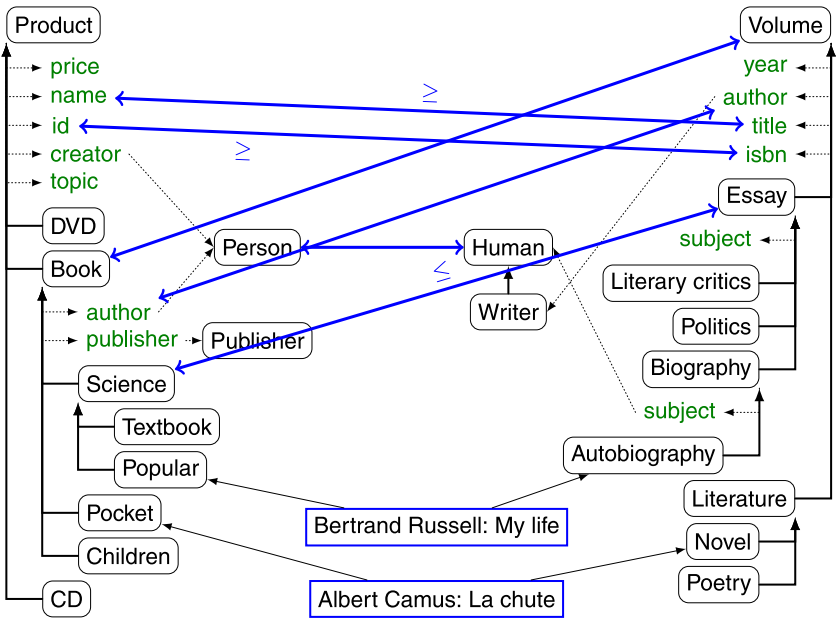
\includegraphics[scale=0.5]{./Fig/Ontologyalignmnet.png}
	\caption{}
	\label{fig:ontologyalognment}
\end{figure}


Ontology matching techniques are based on finding the correspondences between ontologies' entities, structure, or relations. The amount of published research in this area is remarkable. Ontology matching techniques are classified into: string-based, structure-based, constraint-based, instance-based, and model-based techniques. For the purpose of our research, any of state-of-art matching tools could be used. However, we implement the matching technique that we used based on the type of ontology designed and its semantics. 

%However, we implement our matching technique. We used two string similarities, Levenshten ams LCS to map elements between ontologies.

\subsection{Matching Algorithms}

\label {secmatchingalgorithms}

%In this work we used two matching algorithms to measure similarities between ontologyes' components. 

In this section we demonstrate string matching algorithms used in our alignment technique. There are many techniques that could be used to compare strings depending on the way information is represented in the strings. For example, a set of letters, a sequence of letters, an erroneous sequence of letters, a set of words, or a sequence of words. In this work, we used different string similarity measurements. We used Levienshtien distance for sequence of letter strings, longest common subsequence for a sequence of words, Jaccard similarity for a set of words, and SimHash which is based on fingerprint similarity. Other similarity measures could be use for the purpose of matching such as Hamming distance, n-gram similarity, Euclidean, cosine,  Jaro–Winkler, Monge–Elkan, TFIDF and soundex.



\textit{Levenshtein Distance (levDist)}, also called Edit Distance, is defined as the minimum number of insertions, deletions, and substitutions of characters required to transform one string into the other \cite{Levenshtein1966}. Levenshtein Distance provides the minimum total cost of  operations (Op)  between two string as a single number value. We use LevSim (Eq. 1) as a similarity measurement between two strings. this is how to add a citation \cite{Hunt1977} 

% from Hunt1977



\[LevSim(s1,s2 )=1-\cfrac{LevDist(s1,s2)}{max⁡( size(s1),size(s2))}  \qquad    (1) \] 



%In this work we used a different matching algorithms to match components between disassembled code fragments. According to components used in matching we used the algorithm that capture  both syntax and semantic resemblance.

\textit{The Longest Common Subsequence (LCS)} \cite{Hunt1977} algorithm detects the longest common subsequence between two strings. For example, consider the following two sequences of characters.



S1 =\textcolor{red} {A}ABB\textcolor{red} {BCDAB}CD\textcolor{red} {DA}ABD

S2 = DD\textcolor{red} {ABC}CC\textcolor{red} {DA}A\textcolor{red} {B}BB\textcolor{red} {DA}C

For the above example, the LCS among the S1 and S2 sequence is ABCDABDA. For our technique we consider each word as one unit and we used LCS to find the longest common tokens and measure the similarity between two token blocks (Eq. 2).

$$ LCS\_Sim (s1,s2)= \cfrac{LCS(s1,s2)}{\cfrac{size(s1)+size(s2)}{2} }   \qquad  \qquad \qquad   (2)$$

\textit{Jaccard similarity (Jacc)}, also referred to as gloss overlap between two strings, is defined as the intersection of their character set divided by the union of their character set \cite{Jaccard1901} (Eq. 3). We used Jaccard coefficient to measure the similarity (overlap) between two sets of token.  



$$Jacc(s1,s2) =\cfrac{| s1\cap s2  |}{| s1 \cup s2 |}   \qquad  \qquad \qquad \qquad \qquad \qquad \quad  (3) $$ 

\textit{SimHash-based Clone Detection} 
SimHash algorithm constitutes the core of SimCad \cite{Uddin2011}. It generates a 64-bit fingerprint, which we use to detect clones based on their fingerprint similarities. The algorithm uses Charikar's [18] hash function where the Hamming Distance is used as the crucial configuration parameter. The Hamming Distance represents the number of positions at which the corresponding bits are different between two fingerprints. A Hamming distance of zero corresponds to identical fingerprints and therefore also to Type-1 clones, while a Hamming distance larger than zero reflects near-miss clones. 
